\section{Anwendung}

\subsection{Datenkompression \baeni{175}}

\subsubsection{Notation}
\begin{tabular}{ll}
$f$ & diskretes Signal\\
$B$ & Bit-Stream, repräsentiert eine Approximation von $f$ welches mit einer bestimmten Methode codiert wurde. \\
$\tilde{f}$ & Approximation von $f$ repräsentiert durch B, die komprimierte Version von $f$\\
$r$ & Kompressionsrate (zB.: $\dfrac{\text{Anzahl Bits in }f}{\text{Anzahl Bits in }B}$)\\
$\tilde{f}-f$ & Quantisierungsfehler, Quantisierungsrauschen, Verzerrung, Residual\\
\end{tabular}
\begin{tabular}{ll}
$\mathrm{MSE}(\tilde{f}) := \frac{1}{M \cdot N}\sum_{i=0}^{M-1}\sum_{k=0}^{N-1}\lvert \tilde{f}_{i,k}-f_{i,k} \rvert^2$ & Mean Squared Error vom komprimierten Bild\\
$\mathrm{PSNR}(\tilde{f}) := 10 \cdot \log_{10}(\frac{K^2}{\mathrm{MSE}(\tilde{f})})$ & Peak Signal to Noise Ratio, mit $K=\mathrm{max}\{\mathrm{max}(f)-\mathrm{min}(f)\}$ \\
 &  (Bei eine Graustufenbild mit der Farbtiefe 8 beträgt $K=255$)
\end{tabular}

\subsubsection{Vorgehen für Datenkompression}
\[ 
	f \longrightarrow \boxed{\mathrm{Transformation}} \longrightarrow (c_k)_{k\in J} \longrightarrow \boxed{\mathrm{Quantisierung}} \longrightarrow (\tilde{c}_k)_{k \in J} \longrightarrow \boxed{\mathrm{Entropie-Coding}}\longrightarrow B 
\]

Ziel ist es, das Signal $f$ in eine Basis zu transformieren, bei der viel Koeffizienten 0 oder sehr klein werden. Bei der Quantisierung werden diese kleinen Koeffizienten auf 0 quantisiert. Diese Koeffizienten können durch eine effizientes Entropy-Coding komprimiert abgespeichert werden.\\

\textbf{Waveletkompression:}
\begin{itemize}
	\item Das Analyse-Wavelet sollte möglichst viele verschwindende Momente haben, um Anzahl Koeffizienten zu vermindern.
	\item Synthese-Wavelet: Die Synthese-Funktion sollte eine gute Regularität aufweisen, um Artefakte zu vermeiden.
	\item Alle Funktionen sollten symmetrisch sein (gerade oder ungerade, "Lineare Phase"), um Asymmetrien zu vermeiden.
	\item Orthogonalität, um zu verhindern, dass einzelne Koeffizienten zu grosse Fehler verursachen.
	\item Kurze Filter für bessere Performance (Mehr verschwindende Momente und bessere Regularität erhöhen die Filterlänge)
\end{itemize}

\textbf{Bemerkungen:}\\
\begin{itemize}
  \item Ein gutes Wavelet ist das bior4.4. Es ist biorthogonal, symmetrisch, hat 4 vanishing Moments, das Synthese Wavelet hat eine Regularität die grosser als 1.3 ist. Die resultierenden Filter weisen 7 bzw. 9 Filterkoeffizienten auf.
  \item Das Haar-Wavelet hat schlechte Regularität und wenig verschwindende Momente
  \item sym vs bior: bior4.4 hat eine bessere Regularität als sym4 (bessere visuelle Qualität bei einem Bild)
  \item Wavelet mit langen Filtern erzeugen "ringing" an den Kanten (vergleichbar mit Gibbs-Phänomen bei Fourier)
\end{itemize}


\subsubsection{Zwei-Dimensionale Wavelettransformation \baeni{129}}

Die Operatoren $A_k$ berechnet den Approximationskoeffizient der Stufe $k$. Die Detailkoeffizienten der Stufe $k$ werden durch den Operator $D_k^j$ berechnet. Bei den Detailkoeffizienten wird unter horizontal $j=h$, vertikal $j=v$ und diagonalen $j=d$ Details unterschieden. (Horizontal=parallel zur x-Achse)

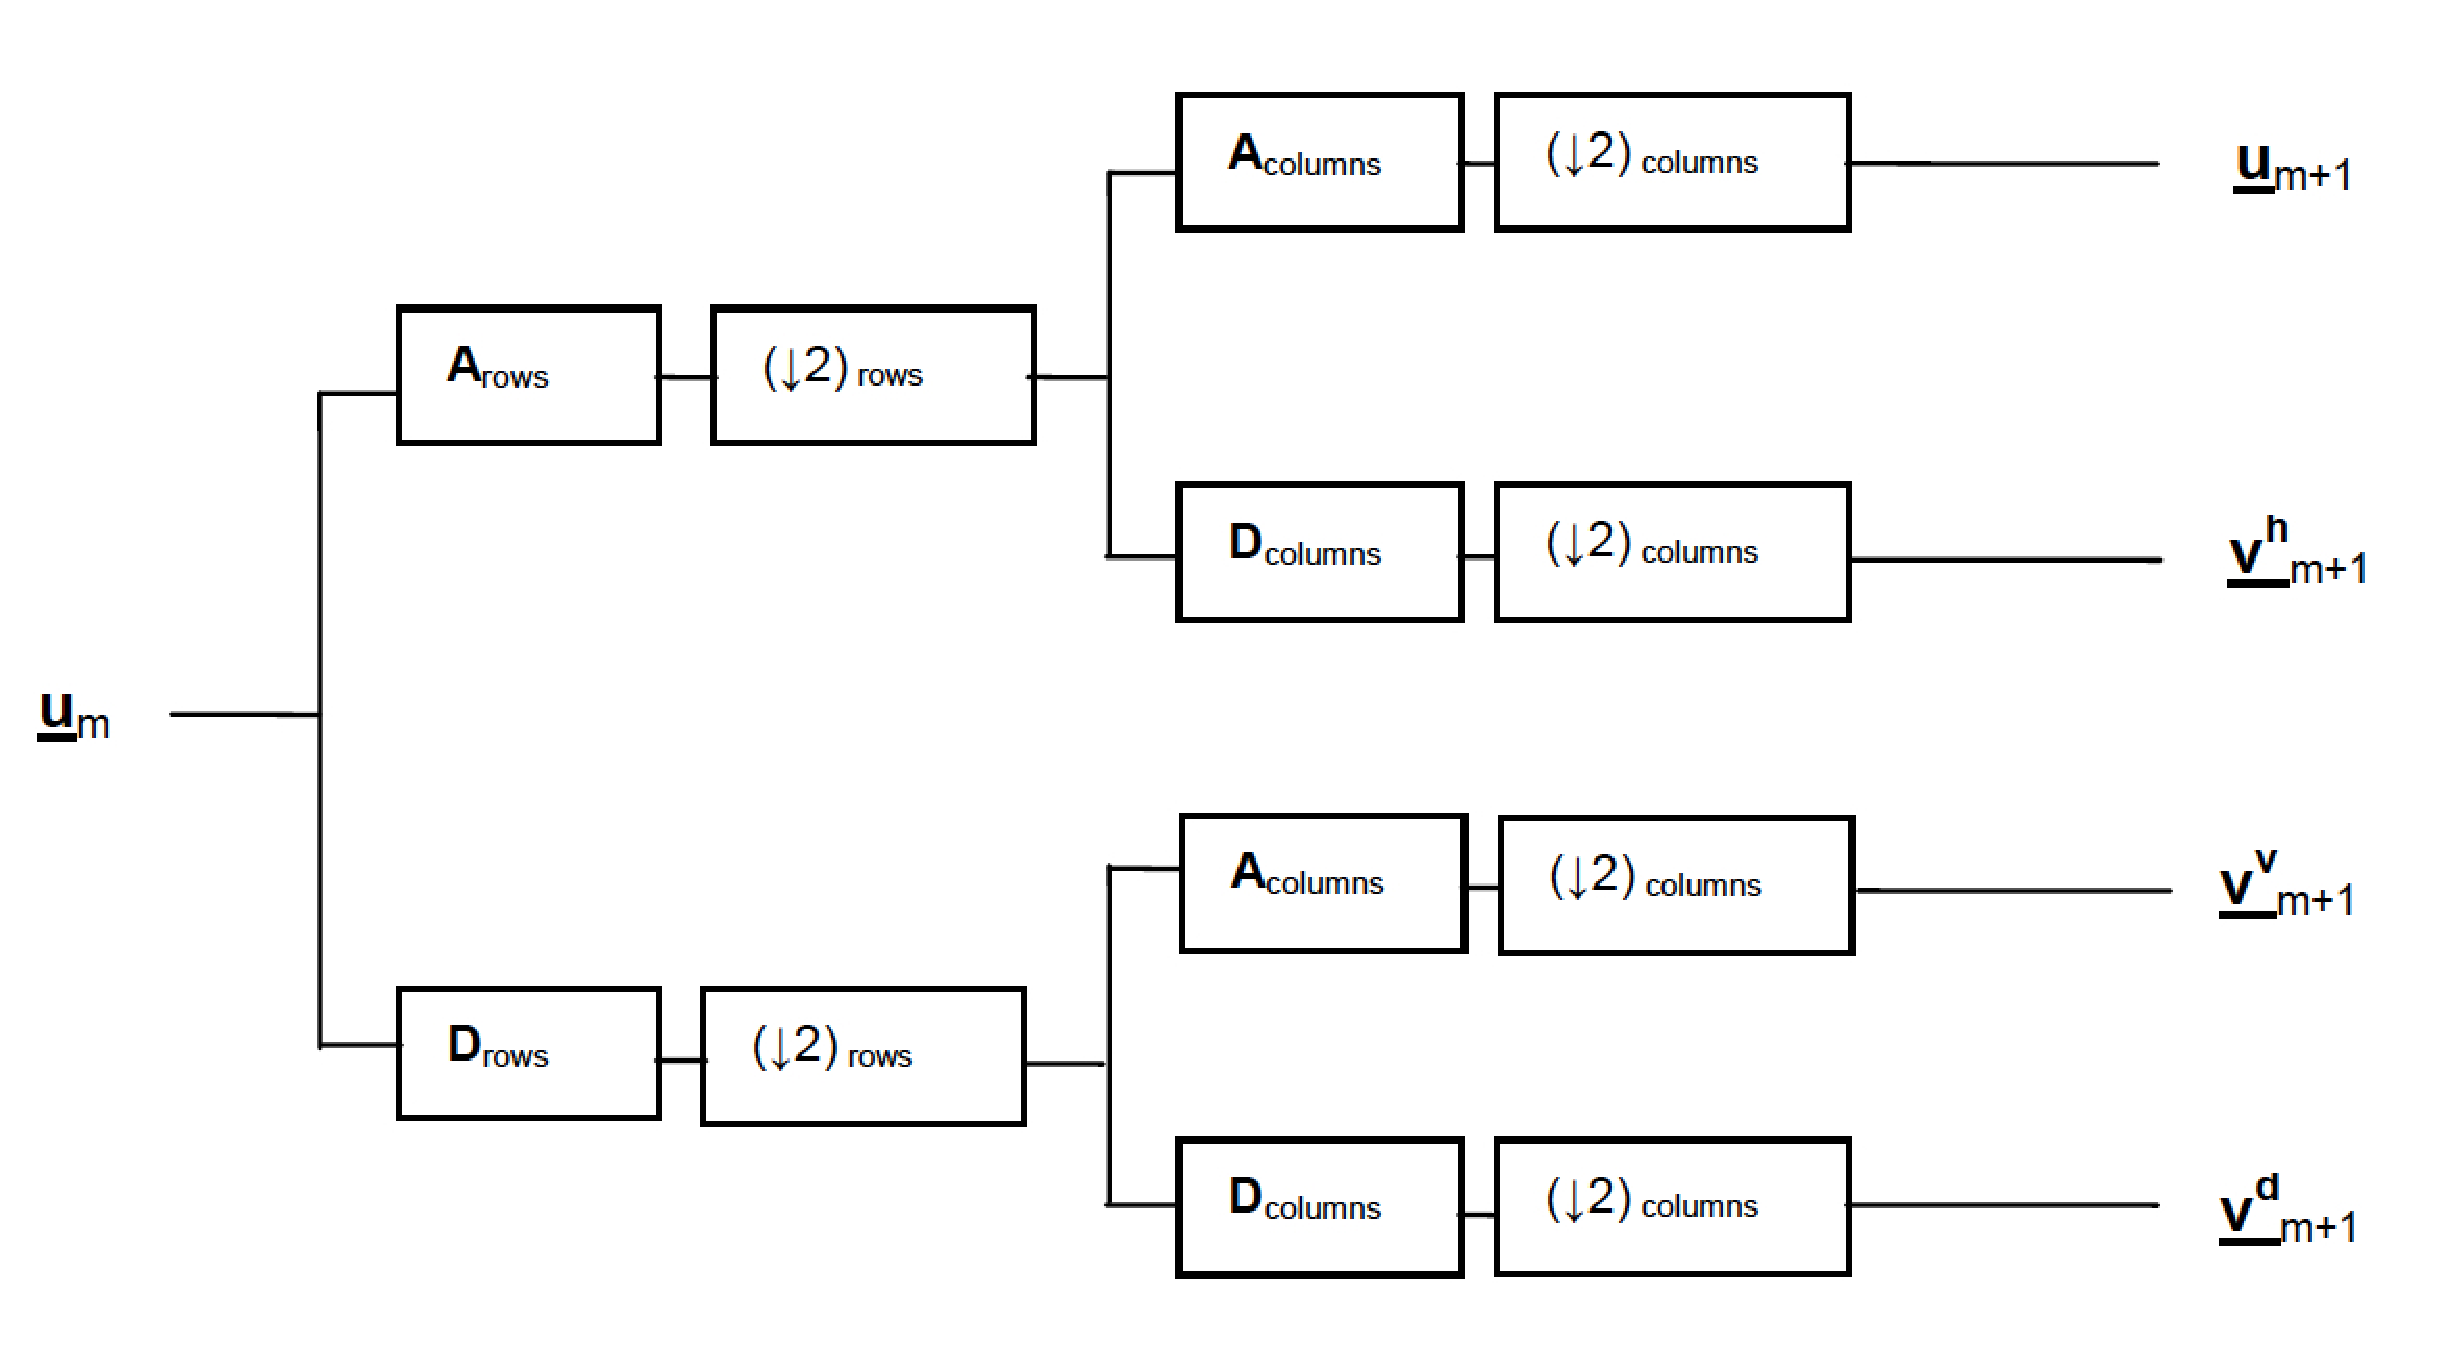
\includegraphics[width=0.5\textwidth]{content/Wavelet2DDec.pdf}	
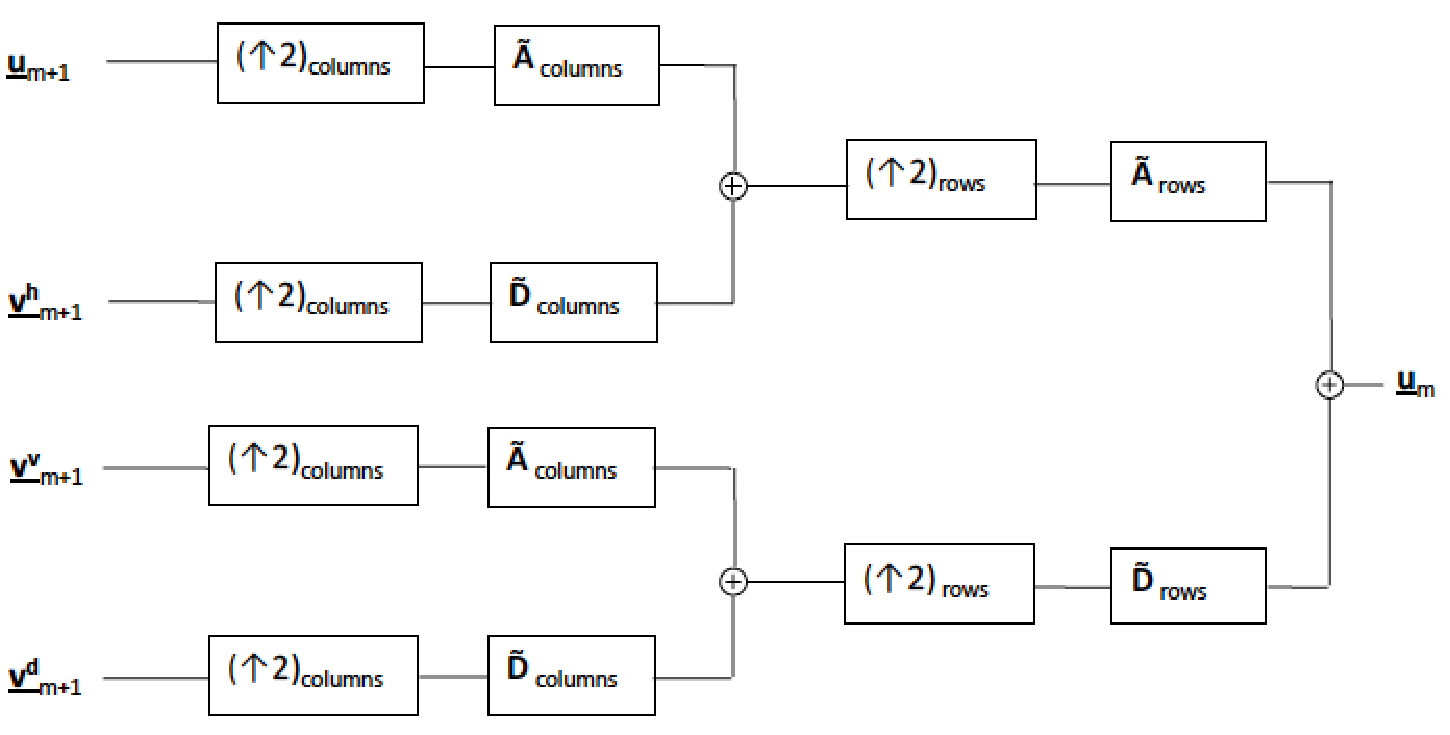
\includegraphics[width=0.5\textwidth]{content/Wavelet2DRec.pdf}

	\[  
		A_0f = A_mf+\sum_{1}^{k=m}(D_k^hf+D_k^vf+D_k^df)
	\]
	\[  
		A_kf(x,y)=\sum_{q\in\mathbb{Z}}\sum_{p\in \mathbb{Z}}u_{k;p,q}\Phi_{k;p,q}(x,y) = \sum_{q\in\mathbb{Z}}\sum_{p\in \mathbb{Z}}u_{k;p,q} \varphi_{k,q}(x) \varphi_{k,p}(y)
	\]
	\[  
		D_k^hf(x,y)=\sum_{q\in\mathbb{Z}}\sum_{p\in \mathbb{Z}}v_{k;p,q}^h\Psi_{k;p,q}^h(x,y) = \sum_{q\in\mathbb{Z}}\sum_{p\in \mathbb{Z}}v_{k;p,q}^h \varphi_{k,q}(x) \psi_{k,p}(y)
	\]
	\[  
		D_k^vf(x,y)=\sum_{q\in\mathbb{Z}}\sum_{p\in \mathbb{Z}}v_{k;p,q}^v\Psi_{k;p,q}^v(x,y) = \sum_{q\in\mathbb{Z}}\sum_{p\in \mathbb{Z}}v_{k;p,q}^v \psi_{k,q}(x) \varphi_{k,p}(y)
	\]
	\[  
		D_d^vf(x,y)=\sum_{q\in\mathbb{Z}}\sum_{p\in \mathbb{Z}}v_{k;p,q}^d\Psi_{k;p,q}^d(x,y) = \sum_{q\in\mathbb{Z}}\sum_{p\in \mathbb{Z}}v_{k;p,q}^d \psi_{k,q}(x) \psi_{k,p}(y)
	\]		
\[ 
	u_{k;q,p}=\langle f|\Phi_{k;q,p} \rangle = \iint_{\mathbb{R}^2} f \cdot \Phi_{k;q,p} \, \mathrm{d}x\mathrm{d}y = \int_{-\infty}^{\infty} \int_{-\infty}^{\infty} f(x,y) \varphi_{k,q} \varphi_{k,p}(y) \, \mathrm{d}x\mathrm{d}y 
\]
\[
	v_{k;q,p}^h=\langle f|\Psi_{k;q,p}^h \rangle = \iint_{\mathbb{R}^2} f \cdot \Psi_{k;q,p}^h \, \mathrm{d}x\mathrm{d}y = \int_{-\infty}^{\infty} \int_{-\infty}^{\infty} f(x,y) \varphi_{k,q} \psi_{k,p}(y) \, \mathrm{d}x\mathrm{d}y \qquad \text{etc.}
\]

Die Filterkoeffizienten werden aber mit der oben abgebildeten Filterbank berechnet.

\begin{center}
	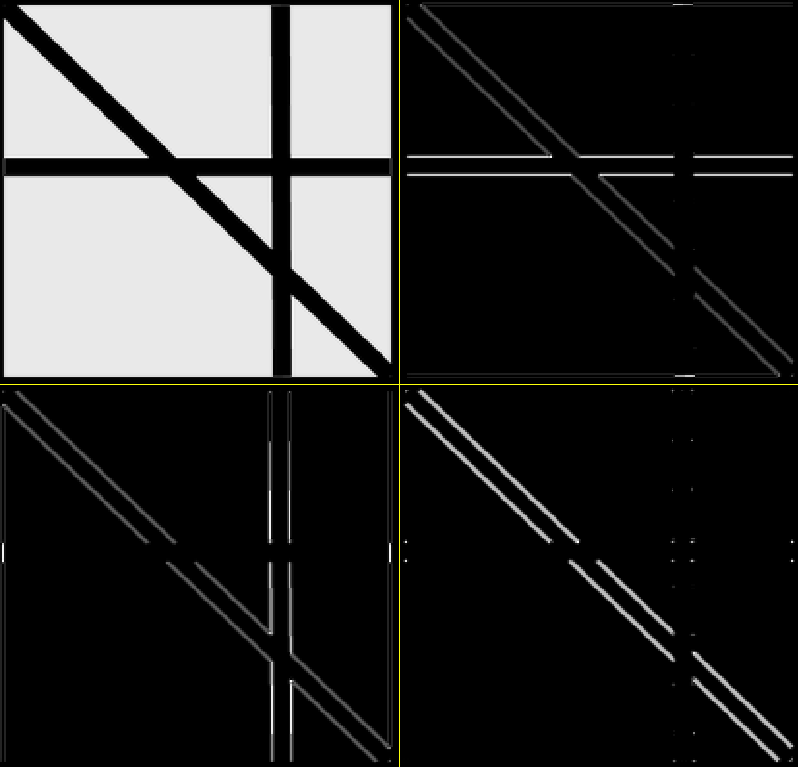
\includegraphics[width=0.35\textwidth]{content/waveBsp2D.png}
\end{center}



\subsection{Denoising \baeni{190}}

\subsubsection{Notation}

\begin{tabular}{ll}
	$f$ & gemessenes Signal (Sequenz von Samples $f_1, f_2,...$), $f=f^\# + f^R$ \\
	$f^\#$ & richtiges Signal (unbekannt) \\
	$f^R$ & Rauschen (unbekannt, stochastisch) \\
	$\tilde{f}$ & Schätzung des richtigen Signals \\
	$\mathrm{MSE}(\tilde{f}) := \frac{1}{N}\sum_{k=0}^{N-1}|\tilde{f}_k - f_k^{\#}|^2$ & Mean Squared Error \\
\end{tabular}

Signal to Noise Ratio (SNR):
\[
	\mathrm{SNR}(\tilde{f}):=10\cdot \log_{10} \left(\frac{1}{N}\sum_{k=0}^{N-1} |f_k^{\#}|^2 / \mathrm{MSE}\right) = \left(\sum_{k=0}^{N-1} |f_k^{\#}|^2 / \sum_{k=0}^{N-1}|\tilde{f}_k - f_k^{\#}|^2\right)
\]

\subsubsection{Vorgehen für Denoising}
\[ 
	f \longrightarrow \boxed{\mathrm{Transformation}} \longrightarrow (v_{m,n}) \longrightarrow \boxed{\mathrm{Thresholding}} \longrightarrow (\tilde{v}_{m,n}) \longrightarrow \boxed{\mathrm{Reconstruction}}\longrightarrow \tilde{f} 
\]

Mit der Annahme, dass die grössten Koeffizienten für die Signalbeschreibung ausreichend sind, kann davon ausgegangen werden das das Rauschen in vielen kleinen Koeffizienten enthalten ist. Ist dies der Fall wird durch Thresholding das Rauschen eliminiert und das wahre Signal nicht gross beeinträchtigt.

Der Vorteil beim Denoising mit Wavelet ist, zum Ersten dass im Zeit- und Frequenzbereich gleichzeitig gearbeitet wird und zum Zweiten dass Signale, die ihre Eigenschaften mit der Zeit ändern, einfach behandelt werden können (zB: Sprünge). 

\vspace{0.5cm}

\begin{minipage}[c]{0.5\textwidth}
	\textbf{Hard-Thresholding} mit der Grenze $\tau$:
	\[ \tilde{v}_{m,n} := \begin{cases} 0 \qquad |v_{m,n}| \leq \tau \\ v_{m,n} \qquad |v_{m,n}| > \tau \end{cases} \]
\end{minipage}
\begin{minipage}[c]{0.5\textwidth}
	\textbf{Soft-Thresholding} (shrinkage) mit Grenze $\tau$:
	\[ \tilde{v}_{m,n} := \begin{cases} 0 \qquad |v_{m,n}| \leq \tau \\ \mathrm{sign}(v_{m,n}) \cdot (|v_{m,n}-\tau|) \qquad |v_{m,n}| > \tau \end{cases} \]
\end{minipage}

Gute Resultate werden unter den folgenden Voraussetzungen erreicht:
\begin{itemize}
	\item das Signal kann vom Wavelet gut komprimiert werden (Wahl des Wavelets)
	\item das Rauschen kann nicht komprimiert werden (Wahl des Wavelets)
	\item SNR($f$) ist genügend gross
\end{itemize}


Wahl von $\tau$, wobei die Schätzung für $\sigma_m$ nur für Rauschen gilt, das gaussverteilte Waveletkoeffizienten aufweist:

\begin{minipage}[c]{0.5\textwidth}
\[
	\tau_m \approx K \cdot \sqrt{2 \cdot \ln(N)} \cdot \sigma_m  
\]
\[
	\sigma_m \approx \dfrac{\mathrm{median}(|v_{m,n}| \, | n \in  \mathbb{Z})}{0.6745} 
\]
\end{minipage}
\begin{minipage}[c]{0.5\textwidth}
$K \in [0.2,1.6]$\\
$N$: Anzahl Samples des Signals $f$\\
median: Ein Wert $m$ ist der Median von einer Menge von Werten wenn die Hälfte aller Werte $\leq m$ und die andere Hälfte $\geq m$ ist. Der Median wird von allen Werten der kleinsten Skalierung genommen (Annahme: Rauschen ist dort am stärksten).
\end{minipage}

\begin{itemize}
	\item White-Noise: Gleiche Grenze $\tau = \tau_1$ in allen Scales ($m=1$ Finest Scale)
	\item Colored-Noise: Die Grenze $\tau$ wird an jede Scale $m$ angepasst.
\end{itemize}


\subsubsection{Stationary  Wavelet Transform (SWT) \baeni{171, 196}}
\begin{tabularx}{\textwidth}{X p{5cm}}

  Die Stationäre Wavelet Transformation ist Translation-Invariant (shift-invariant). Die normale Wavelet Transformation ist nicht Translation-Invariant, dies kommt vom downsamplen. Wenn die Anzahl Scales $J$ ist, kann das Signal $f$ $2^J$ mal verzögert werden, bis wieder das gleiche entrauschte Signal berechnet wird. Aus diesem Grund berechnet die SWT  $2^J$ mal die DWT von verzögerten Signal $f$. Bei alle $2^J$ berechneten DWT wird die Verzögerung rückgängig gemacht und gemittelt. Das dabei entstehende Signal ist die SWT von $f$. 
  & Die nicht-stationäre DWT hat das Problem der Shift-Invarianz:\newline
  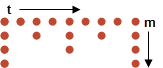
\includegraphics[width=4.5cm]{./content/NonStationarity.png}
\end{tabularx}


\[ 
	\tilde{f}^{tr.inv} := \dfrac{1}{2^J} \sum_{k=0}^{2^J-1}T_k \left( \tilde{T}_k(f) \right) 
	\qquad \qquad
	T_k \text{: delay um $k$-Sample} \qquad \qquad J\text{: Anzahl Scales (Stages, Level)}
\]

Um $\tilde{f}^{tr.inv}$ zu berechnen, steigt die Berechnungszeit um Faktor $2^J$ an. Es gibt effizientere Methoden, bei denen der Aufwand auf Faktor $J$ reduziert werden kann (algorithm à trous, \baeni{171}).

Die SWT lässt das Downsamplen weg, upsampled statt dessen die Filter! Bei der SWT gibt es redundante Informationen über $f$, was schlecht für Kompressionen aber gut für Denoising (smoothing artifacts caused by thresholding) ist.

\begin{minipage}[l]{0.5\textwidth}
	Die dazugehörige Filterbank: \\
	$A_m$ beschreibt den um Faktor 2 upgesampleten Filter $A$ (mit $2^m -1$ Nullen zwischen zwei Filterkoeffizienten eingefügt $(...,a0,0,...,0,a1,0,...,0,a2,0,...)$ )
\end{minipage}
\begin{minipage}[r]{0.5\textwidth}
	\flushright
	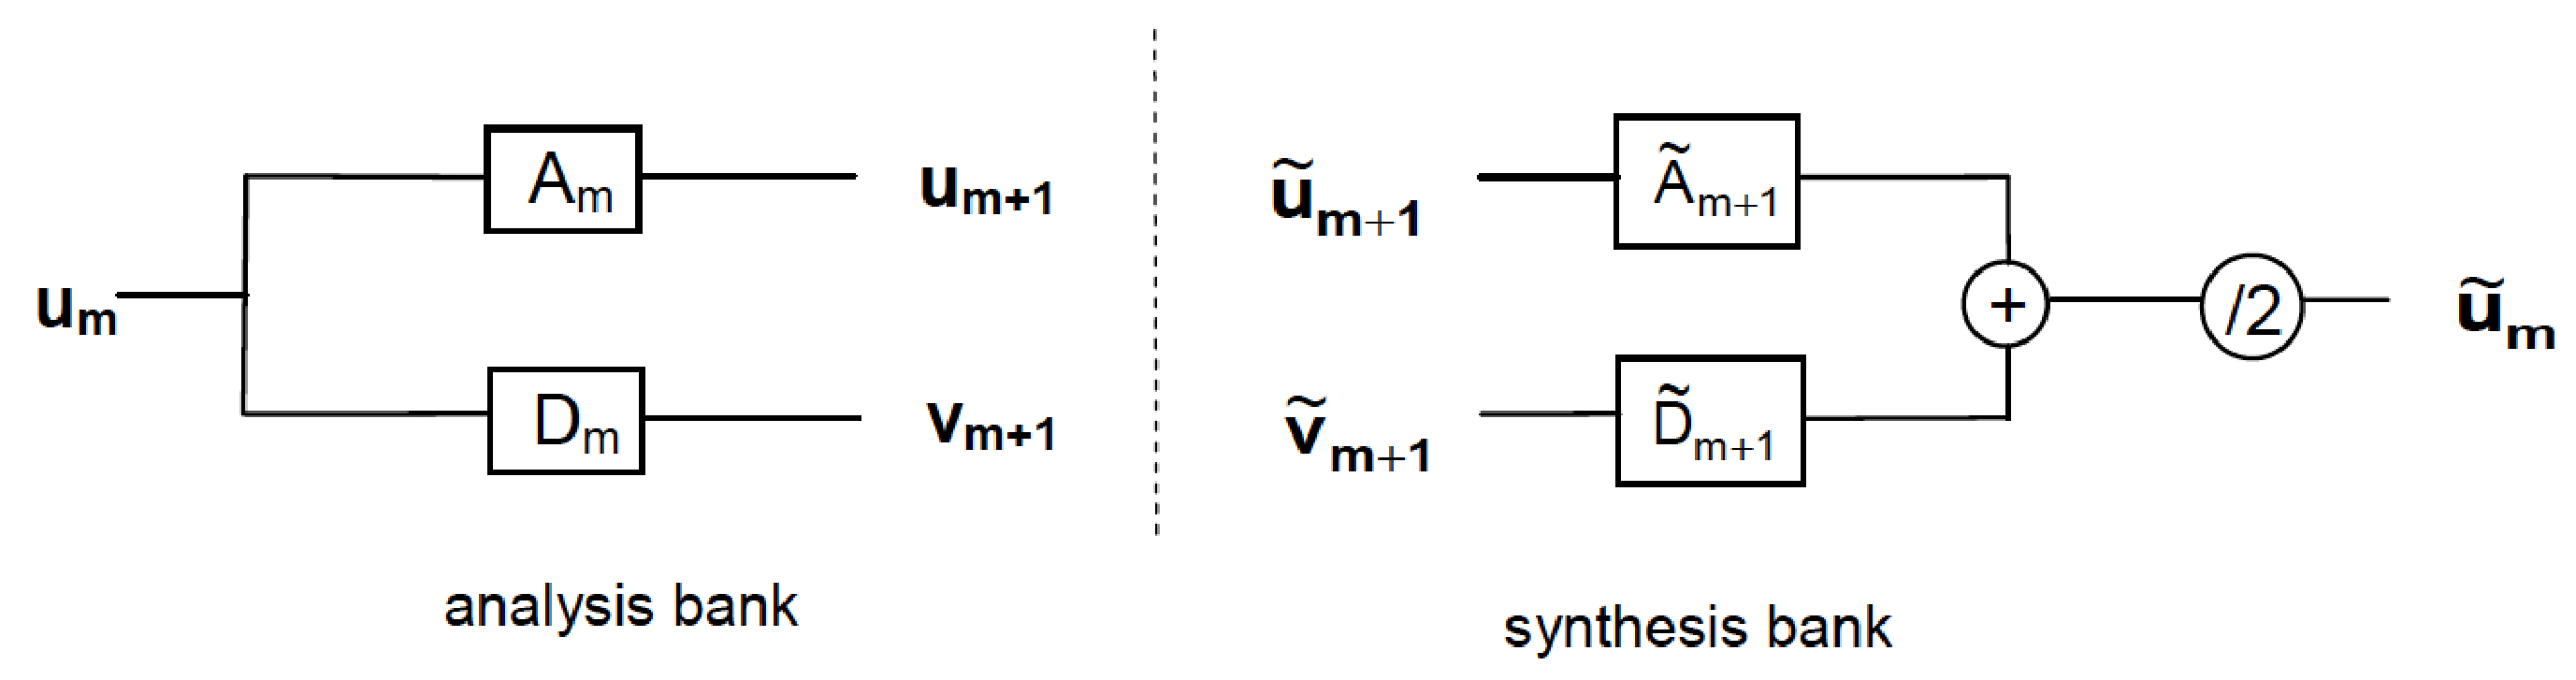
\includegraphics[width=.9\textwidth]{content/swtFilterbank.pdf}
	\[ \tilde{f}^{tr.inv.}=\mathrm{ISWT}(\mathrm{shrink}(\mathrm{SWT}(f)) \]
\end{minipage}


\subsubsection{Abhängigkeit vom MSE und dem Threshold}
\[ MSE(\tilde{f}) = \frac{1}{N} \sum |v_{m,n}|^2 = \frac{1}{N}\left(\underbrace{\sum_{|v_{m,n}| < \tau}|v_{m,n}|^2}_{Rauschenergie} + \underbrace{\sum_{|v_{m,n}| \geq \tau}|v_{m,n}|^2}_{Signalenergie}\right) \]

\newpage
\subsection{Feature Detection and Extraction \baeni{220}}

Feature eines Signals oder eines Bildes ist ein bestimmter Teil Information darin. In 1 Dimension sind dies Peaks, Sprünge oder irgend welche Muster (pattern). Bei Bilder handelt es sich meist um Kanten, Ränder und Ecken.

Feature Detection meint die Lokalisierung der Gebiete wo das Feature auftritt.

FRR: false rejection rate, die W'keit das der Detektor ein Auftretendes Feature übersieht\\
FAR: false acceptance rate, die W'keit das der Detektor ein Feature detektiert das keins ist

\subsubsection{Smooting and Differentiation}
\begin{minipage}[r]{0.5\textwidth}
Smoothing Kernel: $\Theta$\\
Skalierter Smoothing Kernel: $\Theta(\frac{\tau - t}{s})$\\
Smoothed Function: $f_s(t) = \int f(\tau) \cdot \Theta(\frac{\tau - t}{s}) \, \mathrm{d}\tau$\\
Ableitung der Smoothed Function: 
\end{minipage}
\begin{minipage}[r]{0.5\textwidth}
	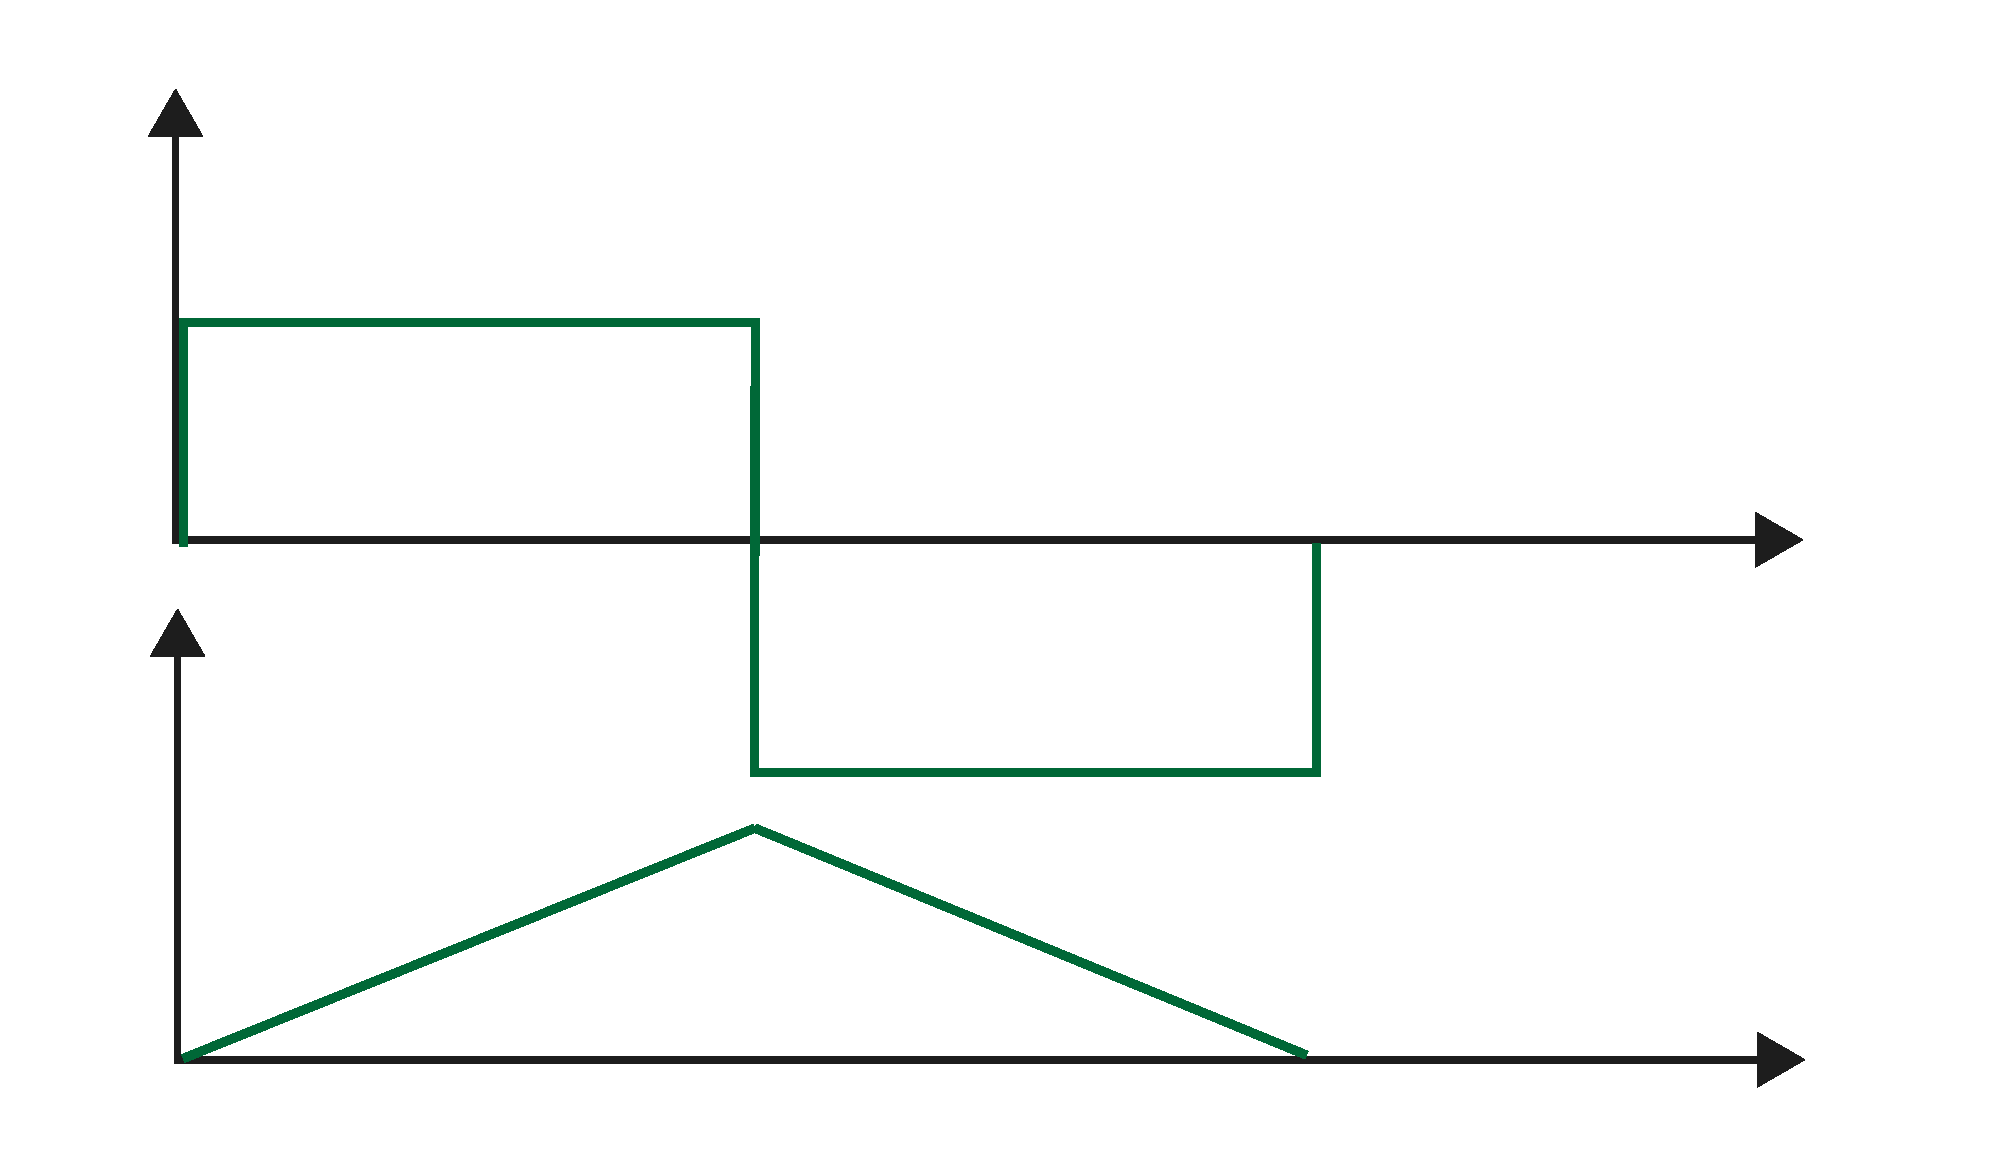
\includegraphics[width=0.4\textwidth]{content/SmoothingFunction.pdf}
	
	\vspace{-2.2cm}
	
	\flushright
	Abgeleiteter Smoothing Kernel
	
	\vspace{.4cm}
	
	Smoothing Kernel	
\end{minipage}

\[ \frac{\mathrm{d}}{\mathrm{d}t}f_s(t) = \int\limits_{-\infty}^{\infty} f(\tau) \cdot \frac{\mathrm{d}}{\mathrm{d}t}\Theta(\frac{\tau - t}{s}) \, \mathrm{d}\tau = -\frac{1}{s} \int\limits_{-\infty}^{\infty} f(\tau) \cdot \Theta'(\frac{\tau - t}{s}) \, \mathrm{d}\tau \]

Wavelet das integriert ein Smoothing Kernel ergibt: Haar-Wavelet ("Abgeleiteter Smoothing Kernel")\\
Daraus Folgt das die DWT oder SWT (besser) für die Approximation der Ableitung der Smoothed Function verwendet werden kann. Wird die SWT verwendet, dann kennt man die Ableitung der Funktion an allen Punkten.
\[ 
	\frac{\mathrm{d}f}{\mathrm{d}t} \approx C(m) \cdot v_{m,n}
	\qquad \qquad
	v_{m,n} =  \int\limits_{-\infty}^{\infty} f(\tau) \psi_{m,n}(\tau) \, \mathrm{d}\tau 
\]
Das Integral vom Smoothing Kernel muss 1 ergeben, damit das Mittel von $f$ gleich bleibt: 
\[ \int \underbrace{\int C(m) \psi_{m,n}(\tau) \,\mathrm{d}\tau}_{\Theta} \,\mathrm{d}t = 1 \]

Das $C(m)$ vom Haar-Wavelet sieht wie folgt aus:
\[
	\frac{1}{C(m)} = \iint \psi_{m,n}(\tau) \,\mathrm{d}\tau \,\mathrm{d}t
	\qquad \Rightarrow \qquad  
	C(m)= 2^{-3m/2 + 2} 
\]

\clearpage
\section{Wavelets und ihre Eigenschaften}


\begin{tabular}{l||l|l|l|l|l|l}
	\textbf{Eigenschaft} & \textbf{haar} & \textbf{dbN}	& \textbf{symN}	& \textbf{coifN} & \textbf{biorNr.Nd}	& \textbf{rbioNd.Nr}	\\
	\hline
	\hline
	Ordnung Decomp.				& 1		& 1,...	& 1,...	& 1-5	& Nd (2)					& Nd (2)	\\
	\hline
	Ordnung Recons.				& 1		& 1,...	& 1,...	& 1-5	& Nr (2)					& Nr (2)	\\
	\hline
	Biorthgonality 				& ja	& ja	& ja	& ja	& ja						& ja		\\
	\hline
	Orthogonality 				& ja	& ja	& ja	& ja	& nein						& nein		\\
	\hline
	Compact support 			& ja 	& ja	& ja	& ja	& ja						& ja		\\
	\hline
	Support width 				& 1 	& 2N-1	& 2N-1	& 6N-1	& rec :2Nr+1, dec: 2Nd+1	& rec :2Nr+1, dec: 2Nd+1	\\
	\hline
	Filter length 				&  2 	& 2N	& 2N	& 6N	& (3) 						& (3)		\\
	\hline
	Regularity 					& nein 	& (1)	& (1)	& (1)	& (4)						& (5)	\\
	\hline
	Symmetry  					& ja 	& nein	& fast	& fast	& ja						& ja		\\
	\hline
	Vanishing moments $\Psi$ 	& 1		& 	N	&	N	& 2N	& Nr						& Nd		\\
	\hline
	Vanishing moments $\Phi$ 	& -		& 	-	&	-	& 2N-1	& - 						& -		\\
\end{tabular}

\vspace{0.2cm}

(1): für grosse N ist das DB Wavelet Regulär! (Regularity: 0.2 N)\\
(2): Nr=1: Nd=1,3,5; Nr=2, Nd=2,4,6,8; Nr=3, Nd=1,3,5,7,9; Nr=4, Nd=4; Nr=5, Nd=5; Nr=8, Nd=8\\
(3): zB: (Nr.Nd: Ld, Lr) 1.3: 6, 2; 2,2: 5, 3 \\
(4): Regularität für Psi bei der rec.: Nr-1 und Nr-2 an den Knoten\\
(5): Regularität für Psi bei der rec.: Nd-1 und Nd-2 an den Knoten

\vspace{0.2cm}

\renewcommand{\arraystretch}{0.1}
\begin{tabular}{l||m{0.3\textwidth}|m{0.3\textwidth}|m{0.3\textwidth}}
	\textbf{Type} & \textbf{Scalingfunction} $\Phi$ & \textbf{Wavelet} $\Psi$ & \textbf{Filtercoeffs}\\
	\hline
	haar & 
	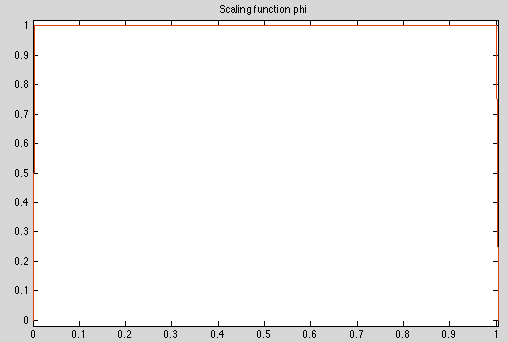
\includegraphics[width=0.3\textwidth]{content/HaarPhi.png} &
	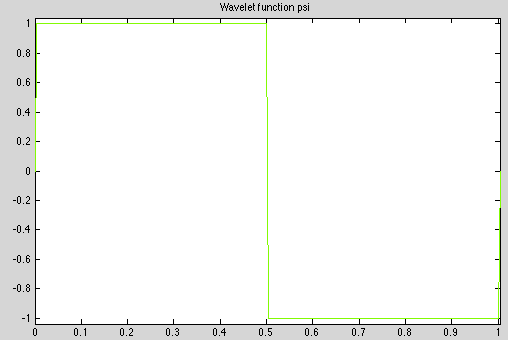
\includegraphics[width=0.3\textwidth]{content/HaarPsi.png} & 
	\begin{align}
		A = \frac{1}{\sqrt{2}} \cdot [\mathbf{1}, 1] \nonumber\\ 
		D = \frac{1}{\sqrt{2}} \cdot [\mathbf{-1}, 1] \nonumber\\
		\tilde{A} = \frac{1}{\sqrt{2}} \cdot [\mathbf{1}, 1] \nonumber\\ 
		\tilde{D} = \frac{1}{\sqrt{2}} \cdot [\mathbf{1}, -1] \nonumber
	\end{align} \\
	\hline
	db2 &
	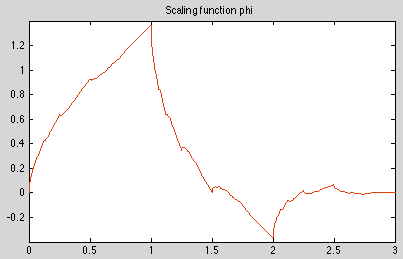
\includegraphics[width=0.3\textwidth]{content/Db2Phi.png} &
	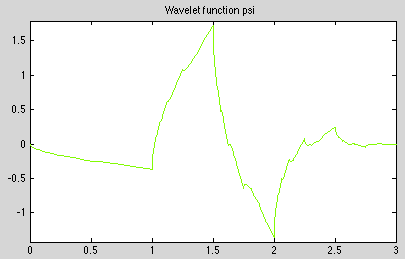
\includegraphics[width=0.3\textwidth]{content/Db2Psi.png} & 
	\begin{align}
		A = \frac{1}{4\sqrt{2}} \cdot [\mathbf{(1+\sqrt{3})}, (3+\sqrt{3}),  \nonumber\\
		(3-\sqrt{3}), (1-\sqrt{3})] \nonumber\\
		D = \frac{1}{4\sqrt{2}} \cdot [\mathbf{(1-\sqrt{3})}, (-3+\sqrt{3}),  \nonumber\\
		(3-\sqrt{3}), (-1+\sqrt{3})] \nonumber\\
		\tilde{A} = \frac{1}{4\sqrt{2}} \cdot [\mathbf{(1-\sqrt{3})}, (3-\sqrt{3}),  \nonumber\\
		(3+\sqrt{3}), (1+\sqrt{3})] \nonumber\\
		\tilde{D} = \frac{1}{4\sqrt{2}} \cdot [\mathbf{(-1-\sqrt{3})}, (3+\sqrt{3}),  \nonumber\\
		(-3+\sqrt{3}), (1-\sqrt{3})] \nonumber
	\end{align} \\
\end{tabular}
\renewcommand{\arraystretch}{1}

\begin{center}
	\begin{tabular}{l||m{0.3\textwidth}|m{0.3\textwidth}}
		Type & Scalingfunction $\Phi$ & Wavelet $\Psi$ \\
		\hline
		db5 &
		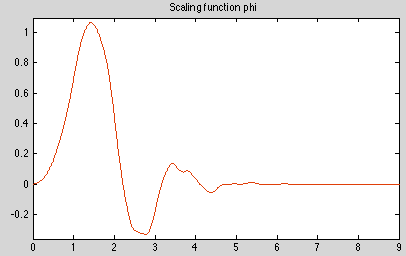
\includegraphics[width=0.3\textwidth]{content/Db5Phi.png} &
		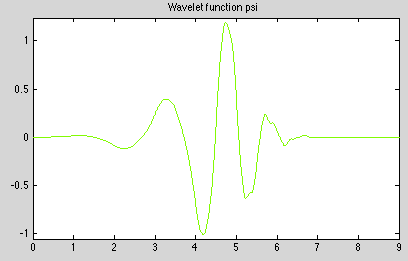
\includegraphics[width=0.3\textwidth]{content/Db5Psi.png} \\
		sym2 & 
		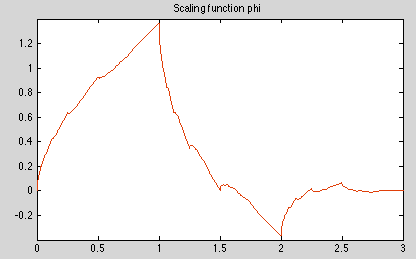
\includegraphics[width=0.3\textwidth]{content/Sym2Phi.png} &
		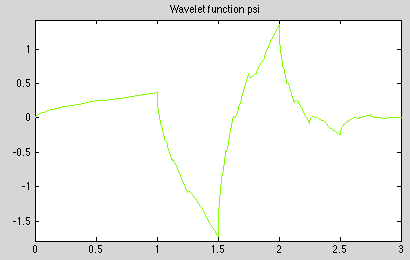
\includegraphics[width=0.3\textwidth]{content/Sym2Psi.png} \\
		sym4 & 
		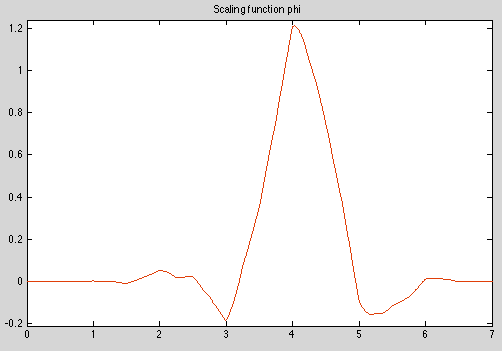
\includegraphics[width=0.3\textwidth]{content/Sym4Phi.png} &
		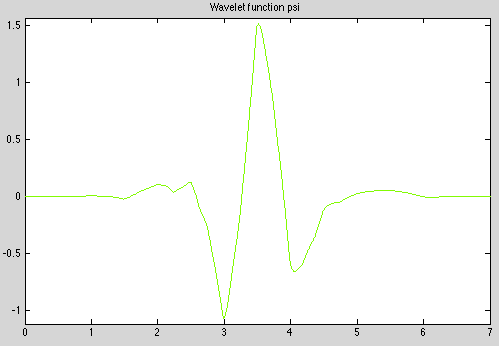
\includegraphics[width=0.3\textwidth]{content/Sym4Psi.png} \\
		coif1 &
		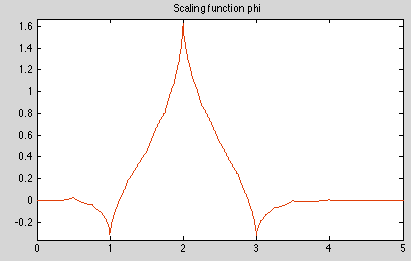
\includegraphics[width=0.3\textwidth]{content/Coif1Phi.png} &
		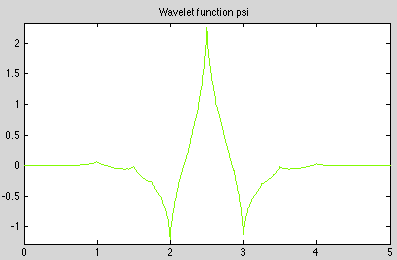
\includegraphics[width=0.3\textwidth]{content/Coif1Psi.png} \\
		coif3 &
		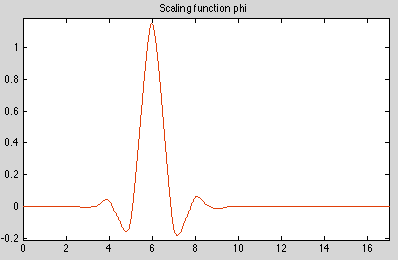
\includegraphics[width=0.3\textwidth]{content/Coif3Phi.png} &
		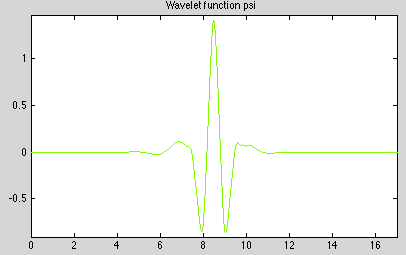
\includegraphics[width=0.3\textwidth]{content/Coif3Psi.png} \\
	\end{tabular}
\end{center}

\textbf{Spezialitäten der Wavelets:}\\
\textbf{db:} grösste Anzahl von vanishing moments für eine gegebene support width, minimum-phase filters\\
\textbf{sym:} beinahe symmetrisch, grösste Anzahl von vanishing moments für eine gegebene support width, near linear-phase filters\\ 
\textbf{coif:} grösste Anzahl von vanishing moments für $\Psi$ und $\Phi$ für eine gegebene support width\\

\begin{center}
	\begin{tabular}{L{0.15\textwidth}||m{0.3\textwidth}|m{0.3\textwidth}}
		Type & Scalingfunction $\Phi$ & Wavelet $\Psi$ \\
		\hline
		bior1.3 (dec.) \newline rbio1.3 (rec.) & 
		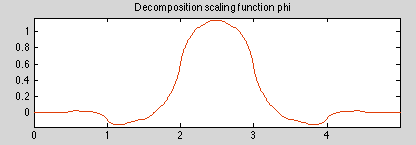
\includegraphics[width=0.3\textwidth]{content/Bior13PhiDec.png} &
		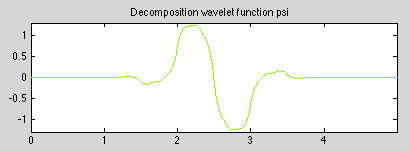
\includegraphics[width=0.3\textwidth]{content/Bior13PsiDec.png} \\
		bior1.3 (rec.) \newline rbio1.3 (dec.) & 
		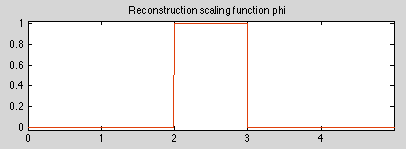
\includegraphics[width=0.3\textwidth]{content/Bior13PhiRec.png} &
		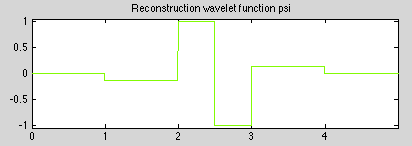
\includegraphics[width=0.3\textwidth]{content/Bior13PsiRec.png} \\
		\hline
		bior2.2 (dec.) \newline rbio2.2 (rec.) & 
		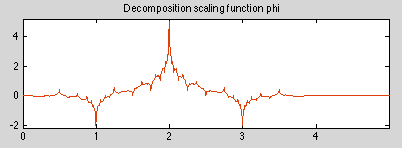
\includegraphics[width=0.3\textwidth]{content/Bior22PhiDec.png} &
		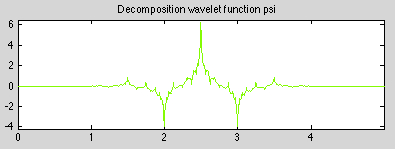
\includegraphics[width=0.3\textwidth]{content/Bior22PsiDec.png} \\
		bior2.2 (rec.) \newline rbio2.2 (dec.) & 
		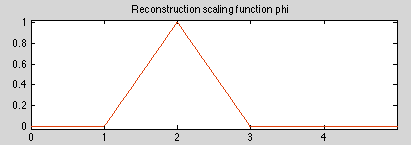
\includegraphics[width=0.3\textwidth]{content/Bior22PhiRec.png} &
		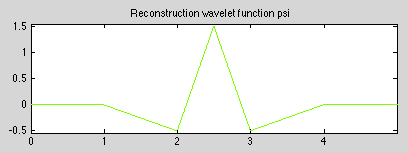
\includegraphics[width=0.3\textwidth]{content/Bior22PsiRec.png} \\
		\hline
		bior4.4 (dec.) \newline rbio4.4 (rec.) & 
		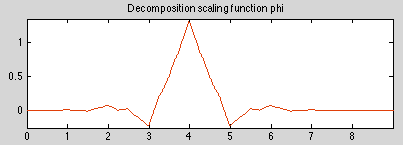
\includegraphics[width=0.3\textwidth]{content/Bior44PhiDec.png} &
		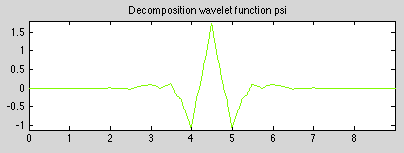
\includegraphics[width=0.3\textwidth]{content/Bior44PsiDec.png} \\
		bior4.4 (rec.) \newline rbio4.4 (dec.) & 
		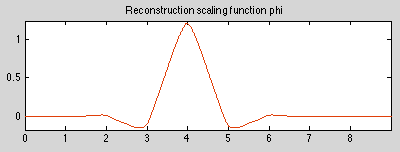
\includegraphics[width=0.3\textwidth]{content/Bior44PhiRec.png} &
		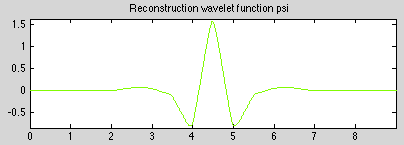
\includegraphics[width=0.3\textwidth]{content/Bior44PsiRec.png} \\
	\end{tabular}
\end{center}

\textbf{Spezialitäten der Wavelets:}\\
\textbf{bior, rbio:} symmetrisches biorthogonal spline wavelet, exakter Rekonstruktion, mit FIR Filter (orthogonal ist dies nur mit dem Haar Wavelet möglich)





\newpage
\subsection{Matlab} 

\subsubsection{Wavelet Decomposition and Reconstruction}
Im folgenden Matlabcode wird die Wavelet Decomposition (wavedec) und die Wavelet Reconstruction (waverec) über eine Stufe mit der Faltung (conv) der Filterkoeffizenten und dem Signal durchgeführt.
\lstinputlisting[language=Matlab]{content/waveDecRecSelf.m}



\subsubsection{Feature Detection}
\textbf{Ableitung:}

\vspace{-0.4cm}

\begin{lstlisting}[language=Matlab]
	function [ cm ] = C( m )
		cm = 2^(-3*m/2+2);
	end
\end{lstlisting}

\lstinputlisting[language=Matlab]{content/derivative.m}

Für die zweite Ableitung kann das Resultat der derivative Funktion einfach nochmals an diese übergeben werden.



\subsubsection{Denoising}

\textbf{Noise:}

\vspace{-0.4cm}

\begin{lstlisting}[language=Matlab]
	r = randn(1,N); %generate uniform or gaussian noise
	r1 = r(2:end)-r(1:end); %colored noise (more noise at high f)
	r2 = r(2:end)+r(1:end); %colored noise (more noise at low f)
\end{lstlisting}

\textbf{DWT:}\\
Mit konstantem Sigma über alle Level:

\vspace{-0.4cm}

\lstinputlisting[language=Matlab]{content/denoise.m}

Mit angepasstem Sigma pro Level:

\vspace{-0.4cm}

\lstinputlisting[language=Matlab]{content/estimateSigmaByLevel.m}
\newpage
\lstinputlisting[language=Matlab]{content/denoiseGivenSigma.m}

\newpage
\textbf{SWT:}

\vspace{-0.4cm}

\lstinputlisting[language=Matlab]{content/stationaryWaveletTransform.m}
\lstinputlisting[language=Matlab]{content/denoiseSwt.m}

